\documentclass[a4paper]{article}

\usepackage[english]{babel}
\usepackage[utf8]{inputenc}
\usepackage{amsmath}
\usepackage{graphicx}
\usepackage[colorinlistoftodos]{todonotes}
\usepackage{listings}
\usepackage{float}
\title{Estimate parameters of AR model}

\author{Vladislav Iliushin}

\date{\today}

\begin{document}
\maketitle

 

\section{Data initialization}
Because  WAVREAD will be removed in a future release we will use AUDIOREAD instead:
\begin{verbatim} [y,Fs]=audioread('gong.wav');
 \end{verbatim}

\section{Problem definition}
\subsection{Ma $\approx{}$ b}



\[ \left. M =\begin{pmatrix}
 1 & y_{p-1}&  \cdots& y_{0} \\ 
 \vdots  &  \vdots&   \vdots & \vdots \\ 
 1 &  y_{T-1} & \cdots & y_{T-p}
\end{pmatrix} \right.
%
\left. b =\begin{pmatrix}
y_{p}\\ 
y_{p+1}\\
\vdots \\ 
y_{T}
\end{pmatrix} \right.
\]

Or, considering Matlab indexing:

\[ \left. M =\begin{pmatrix}
 1 & y_{p}&  \cdots& y_{1} \\ 
 \vdots  &  \vdots&   \vdots & \vdots \\ 
 1 &  y_{T} & \cdots & y_{T-p+1}
\end{pmatrix} \right.
%
\left. b =\begin{pmatrix}
y_{p+1}\\ 
y_{p+2}\\
\vdots \\ 
y_{T+1}
\end{pmatrix} \right.
\]


\subsection{ $\textup{min}_{\mathbf{a}} \left \| \mathbf{ Ma-b }\right \|^{2} $}
\[\textup{min}_{\mathbf{a}} \parallel\mathbf{ Ma-b }\parallel^{2} = 0.0020867\]

\section{Problem definition using QR decomposition}
\subsection{$\textup{x}=\textup{solve}\_\textup{ls}(\textup{A},\textup{b})$}

\begin{verbatim} 
	function x = solve_ls(  A, b )
	% size
    s = size(A, 2);
    % QR Decomposition
    [Q, R] = qr(A, 0);  
    % Least squares
    bq = Q' * b;
    x = zeros(s, 1);
    for i = s:-1:1
        x(i) = (bq(i) - (R(i,:) * x)) / R(i, i);
    end
	end
 \end{verbatim}
 \subsection{ $\textup{ Distance} \left \| \widehat{a_{1}} -\widehat{a_{2}} \right \| $}
\[\left \| \widehat{a_{1}} -\widehat{a_{2}} \right \| = 5.3075\cdot 10^{-12}\]

\section{Synthetic sound generation}
\subsection{Sound reconstruction}

\[y_{syn\_t} = y_{orig\_t},    0 \leq t < p\]
\[y_{t} = a_{0} + \sum_{i=1}^{p} a_{i}y_{t-i}+\varepsilon_{t}, t < p\]
%
Or, considering Matlab indexing: 
%
\[y_{syn\_t} = y_{orig\_t},    1 \leq t < p+1\]
\[y_{t} = a_{1} + \sum_{i=2}^{p+1} a_{i}y_{t-i+1}+\varepsilon_{t} t\geq p\]
\subsection{Sound comparation}

\begin{figure}[H]
	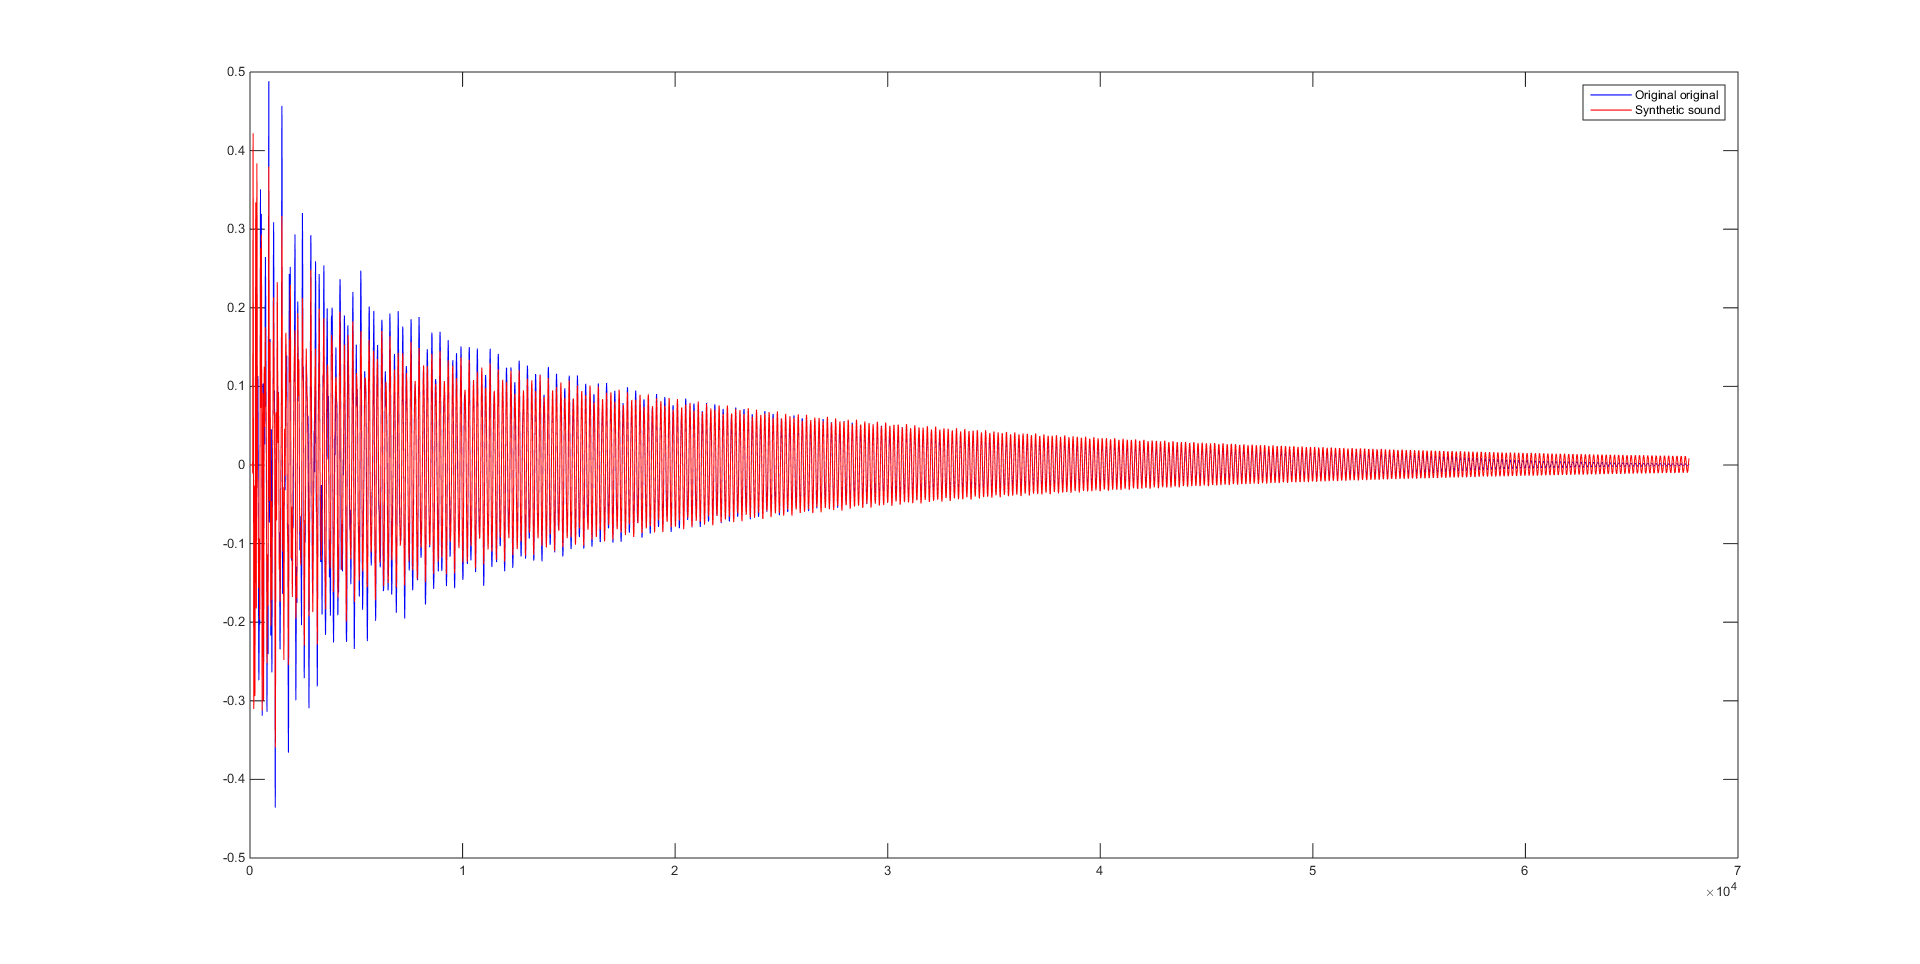
\includegraphics[scale=0.3]{comparation_ab.png}
	\caption{Comparation between original sound and synthetic sound, generated using least squares}  
    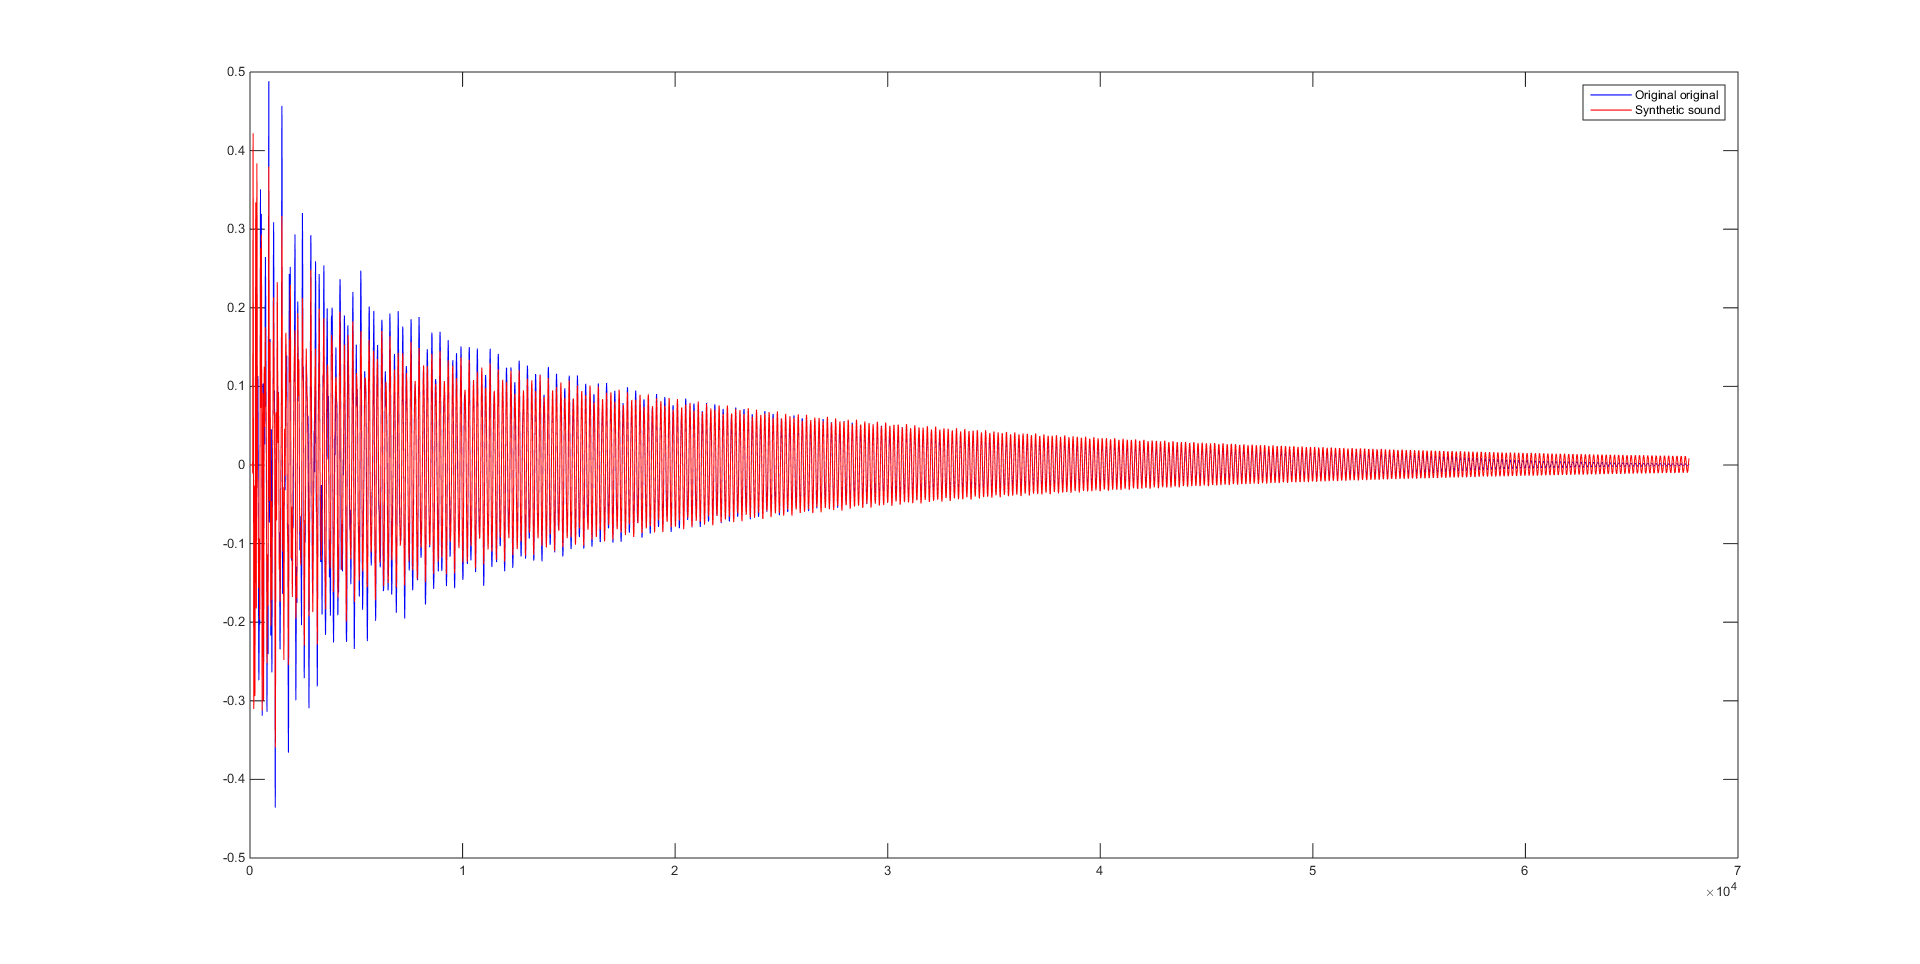
\includegraphics[scale=0.3]{comparation_qr.png}
	\caption{Comparation between original sound and synthetic sound, generated using QR decomposition}
   
\end{figure}


\end{document}